\chapter{Development}\label{sec:cap3}

This chapter describes the development of the anomaly detection system, which aims to create a toolkit for anomaly detection, model training, and comparison between different models. The toolkit is designed to be modular, allowing for easy integration of new models and features.

\section{System Design}

The anomaly detection system is composed by independent nodes. There is a central node that orchestrates the system, and several nodes that implement the anomaly detection models. Each model node works as a microservice and is responsible for training and predicting anomalies using its own algorithm. The central node is responsible for managing the data flow between the model nodes and the outlier protocol. The system design is shown in \autoref{fig:system-design}.

\begin{figure}[H]
    \centering
    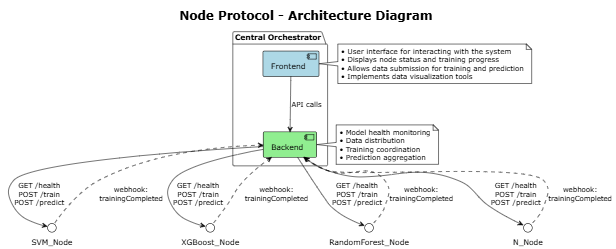
\includegraphics[width=\textwidth]{system-arch.png}
    \caption{Anomaly detection system design}
    \label{fig:system-design}
\end{figure}

\section{Outlier Protocol}

The outlier protocol is a custom protocol based on the OpenAPI specification. It is a simple protocol that describes how the orchestrator interacts with the model nodes, and is based on HTTP messages, which can be grouped into three main categories: \textit{health}, \textit{train}, and \textit{predict}.

The current implementation is based on offline data, and a preprocessing is required in order to transform real data to the model's accepted one. This preprocessing consists on \todo{acotar} the discharge (delete everything before the beginning of the experiment, as sensors might be activated from before), and to \todo{remuestrear} data to a constant rate (1 or 2 ms accepted).

\subsection{Health}

Models must implement the \texttt{/health} endpoint in order to be visible to the orchestrator. The orchestrator will send a \texttt{GET} message at a variable time. If the model does not answer, orchestrator must consider the model as unavailable, and data must not be sent to this model.\ \autoref{fig:health-message} shows the sequence diagram of the health message and its response. This message also includes the model name, uptime, and last training time.

\begin{figure}[H]
    \centering
    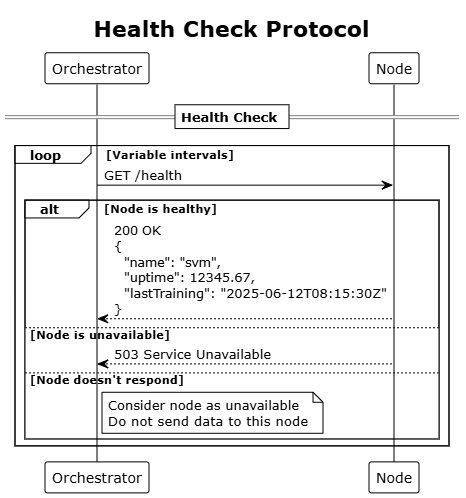
\includegraphics[width=0.75\textwidth]{health.png}
    \caption{Health message sequence diagram}
    \label{fig:health-message}
\end{figure}

\subsection{Train} 

This category describes how models will be trained in order to acquire data for disruption prediction. 

Protocol begins with a \texttt{post} message to the \texttt{/train} model endpoint that contains the number of discharges that will be sent to the models. Models that want to accept the training, answer with a 200 response. Then the orchestrator sends, one by one, the training discharges. After a discharge is received, models must acknowledge it. When all discharges are sent, models shall start the training.

When the training is done, models must inform the orchestrator, as shown in \autoref{fig:train-message}.

\begin{figure}[H]
    \centering
    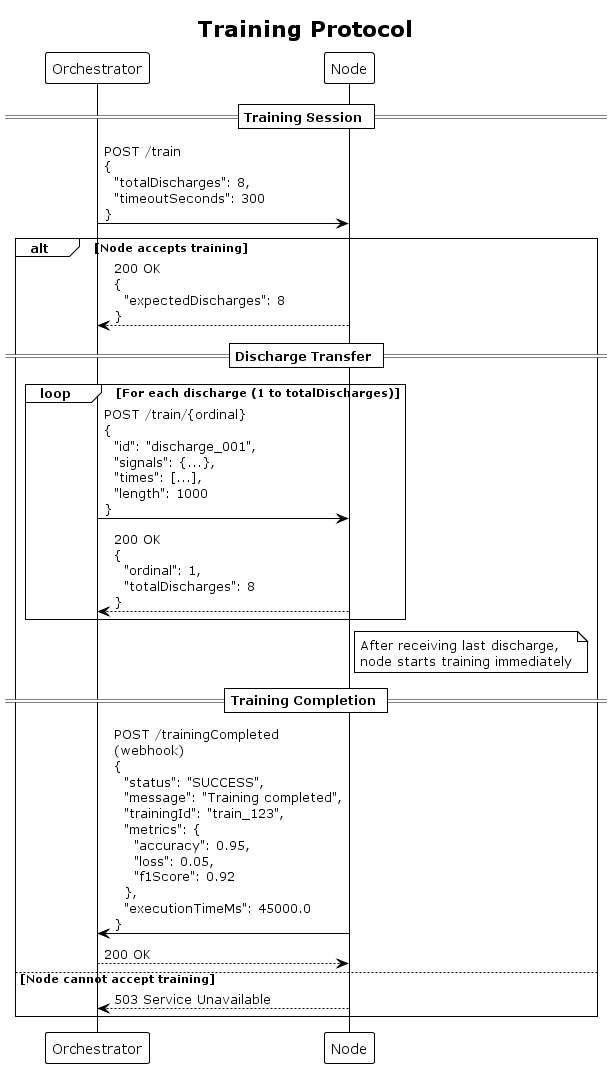
\includegraphics[width=0.75\textwidth]{train.png}
    \caption{Train message sequence diagram}
    \label{fig:train-message}
\end{figure}

\subsection{Predict}
\todo[inline]{Actualizar la figura de predict. En el outlier protocol no están puestas las features que se deben enviar.
\href{https://github.com/outlierClassifier/outlier_protocol/issues/3}{GH issue 3}}

The \texttt{predict} message is sent by the orchestrator to the alive models. It is a \texttt{POST} message to the \texttt{/predict} model endpoint and simulates online data. For this reason, models must send a prediction per window and the features that have been taken into account for the decision. Models must also report a \textit{justification} value, which is the confidence of that window to belong to a class.

\missingfigure{Prediction response message sequence diagram}

\section{Outlier Orchestrator}\label{sec:orchestrator}

The outlier orchestrator is the central node of the anomaly detection system. It is responsible for managing the data flow between the model nodes, using the outlier protocol to communicate with them.

The orchestrator consists on a frontend and a backend. The frontend is a web application that allows users to interact with the system, while the backend is responsible for managing the data flow and the communication with the model nodes.

The frontend is built using HTML, CSS, and JavaScript, and provides a user-friendly interface for managing the models and the data. It allows users to start and stop the models, view the health status of the models, and visualize the results of the anomaly detection.

The backend is built using Node.js, which is a JavaScript runtime that allows to run JavaScript code on the server side.

Communication between the frontend and the backend is done throw \texttt{Socket.io}, which is a library that allows real-time communication between the client and the server. This allows the frontend to receive updates from the backend in real-time, such as the health status of the models or the results of the anomaly detection.

\subsection{Frontend}

The frontend main page is shown in \autoref{fig:frontend-main}. There are two main panels: the top panel shows the available models, and the bottom panel consists on four tabs: \textit{Prediction}, \textit{Training}, \textit{History}, and \textit{Preview}.

\begin{figure}[H]
    \centering
    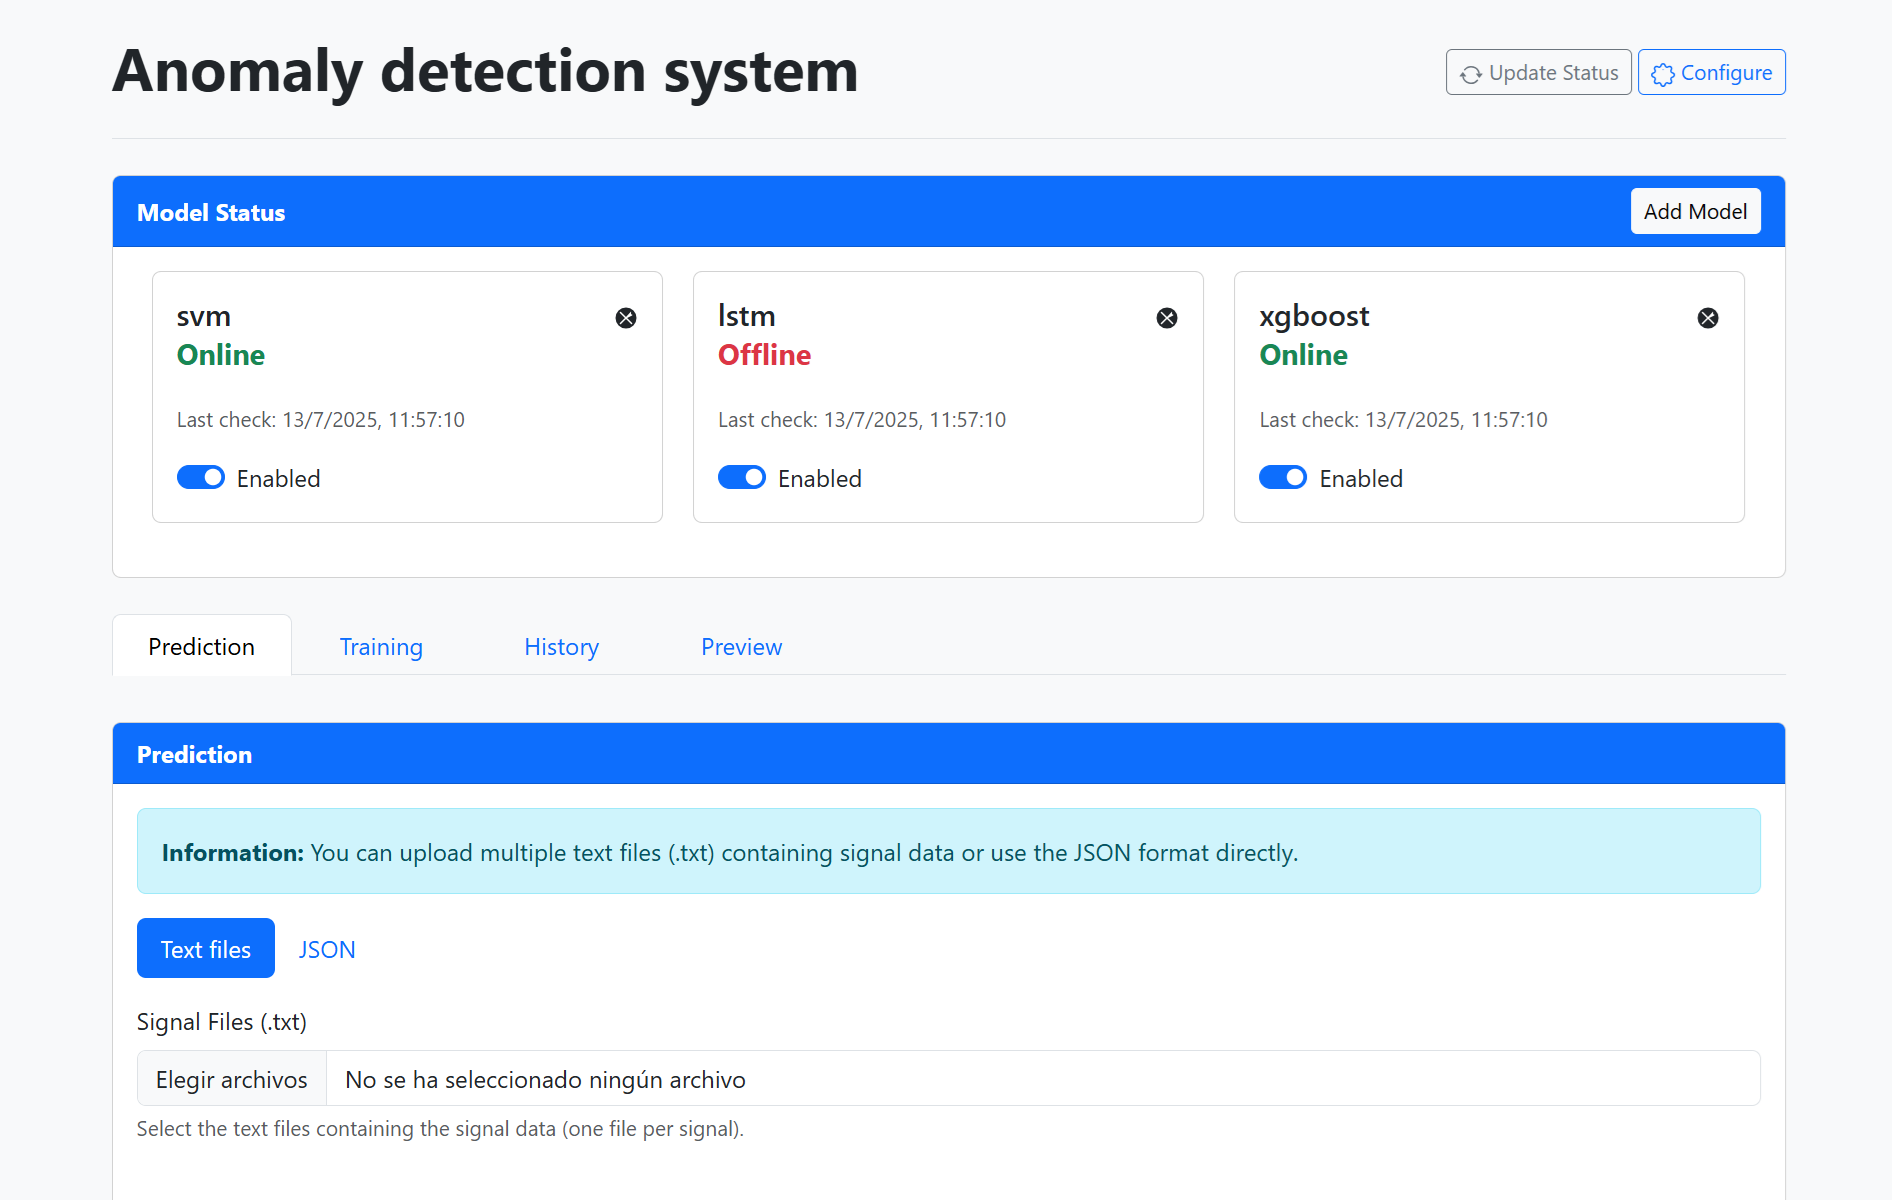
\includegraphics[width=\textwidth]{frontend-principal.png}
    \caption{Frontend main page}
    \label{fig:frontend-main}
\end{figure}

The backend is responsible for sending the model status to the frontend, including the health status, the training status and the prediction results, while the frontend is responsible of displaying this information to the user and sending the backend the user actions, such as adding or removing models, enabling or disabling models, changing model endpoints, starting a training, or making a prediction.

Model configuration is done through the \textit{Configure} button, which opens a modal where the user can change the model's endpoints. This modal is shown in \autoref{fig:frontend-configure}.

\begin{figure}[H]
    \centering
    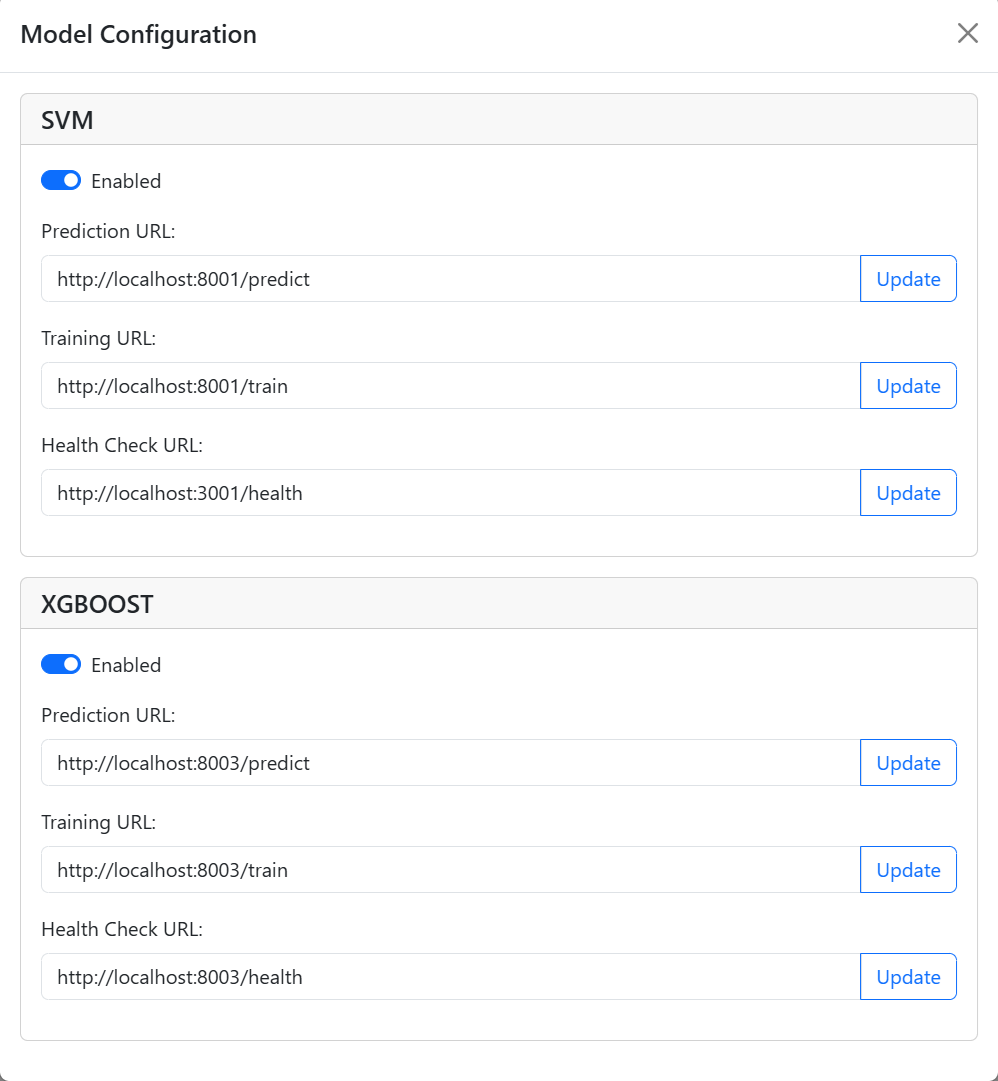
\includegraphics[width=0.5\textwidth]{model-configuration-modal.png}
    \caption{Model configuration modal}
    \label{fig:frontend-configure}
\end{figure}

\subsubsection{Prediction Tab}

The prediction tab allows users to make predictions using the available models. It provides a simple interface where users can choose the discharge to analyze. The \autoref{fig:frontend-prediction} shows the prediction tab and the result of a prediction.

\begin{figure}[H]
    \centering
    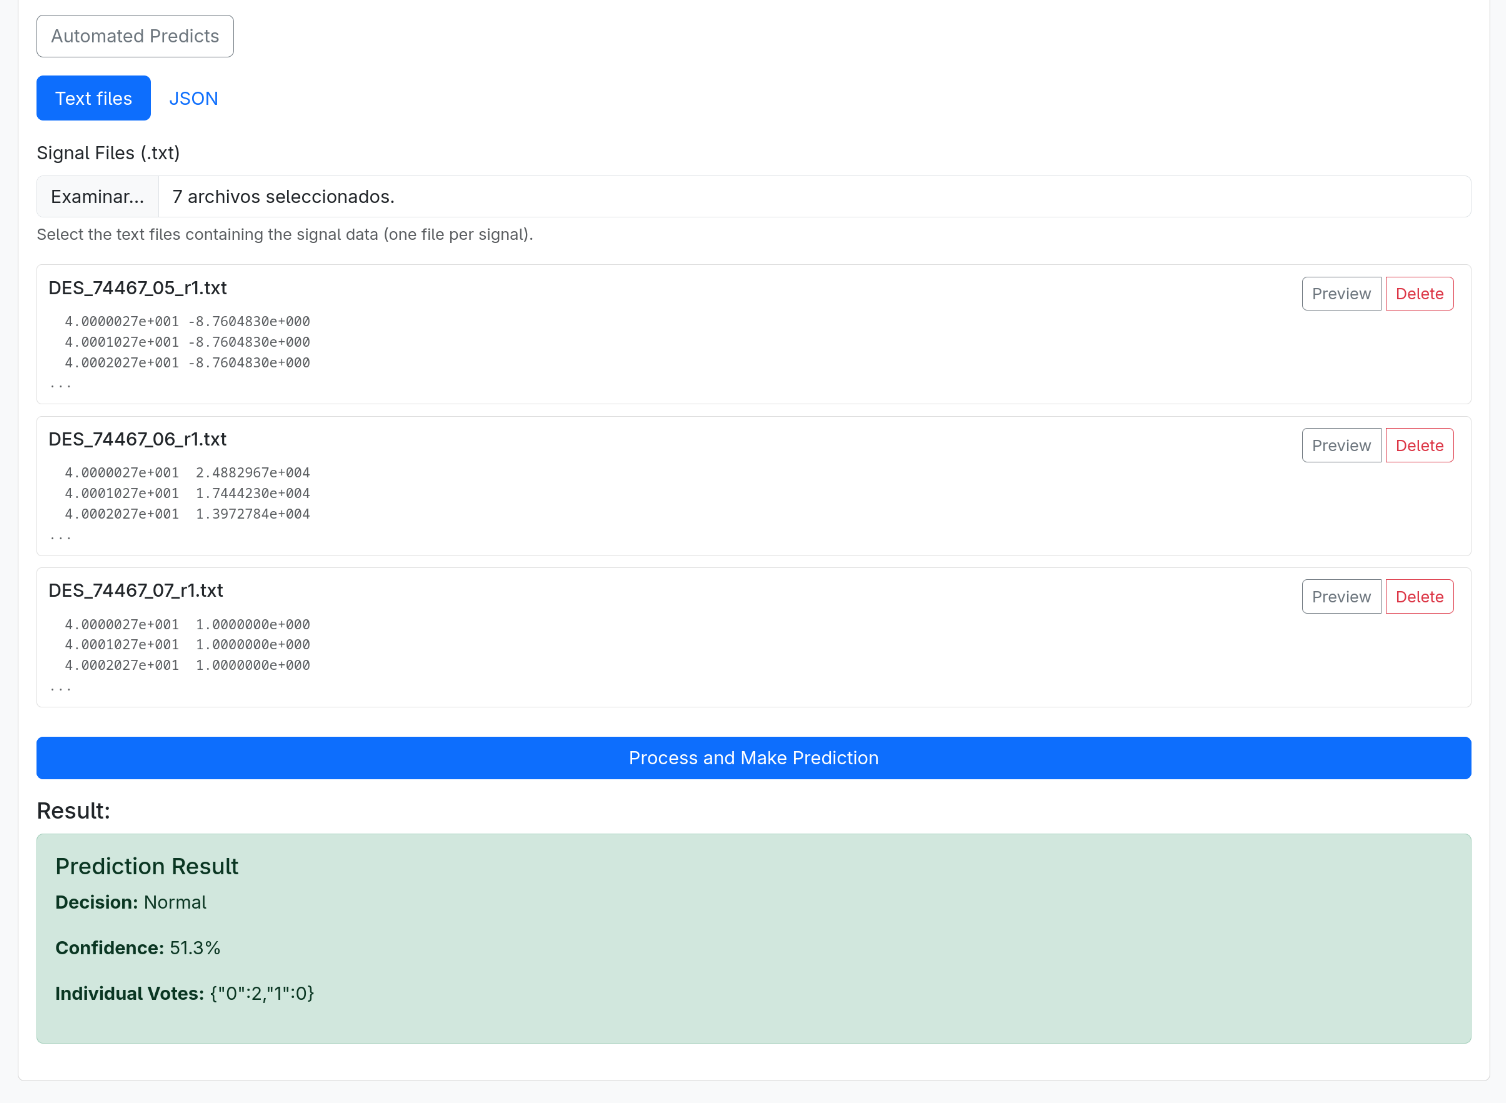
\includegraphics[width=\textwidth]{frontend-prediction.png}
    \caption{Frontend prediction tab}
    \label{fig:frontend-prediction}
\end{figure}

To ease models comparison, prediction orders can be automatically sent for discharges on a folder. As the Outlier Protocol specifies, models must report prediction per window, and add a justification. But models can differ in how do they calculate the final result. For example, as explained on \autoref{sec:models}, SVM calculates the distance to the separation hyperplane, and it is considered disruption if this value is positive, while XGBoost calculates a probability for being disruptive, so a value between 0 and 1 is returned. For this reason, user can set a threshold for a model, which is the first justification value that will be considered disruptive. Also, a \textit{count threshold} can be specified, this is, the number of consecutive windows that need to be labeled as disruptive to consider that discharge as disruptive. This behavior is represented on \autoref{fig:auto-pred}. The modal enables these personalization options for every online model. 

The frontend excludes the unwanted files and fetches the backend's \texttt{/api/ automated-predicts/session} endpoint, which handles user's information. On the backend section there is a detailed explanation of the implementation.

\begin{figure}[H]
    \centering
    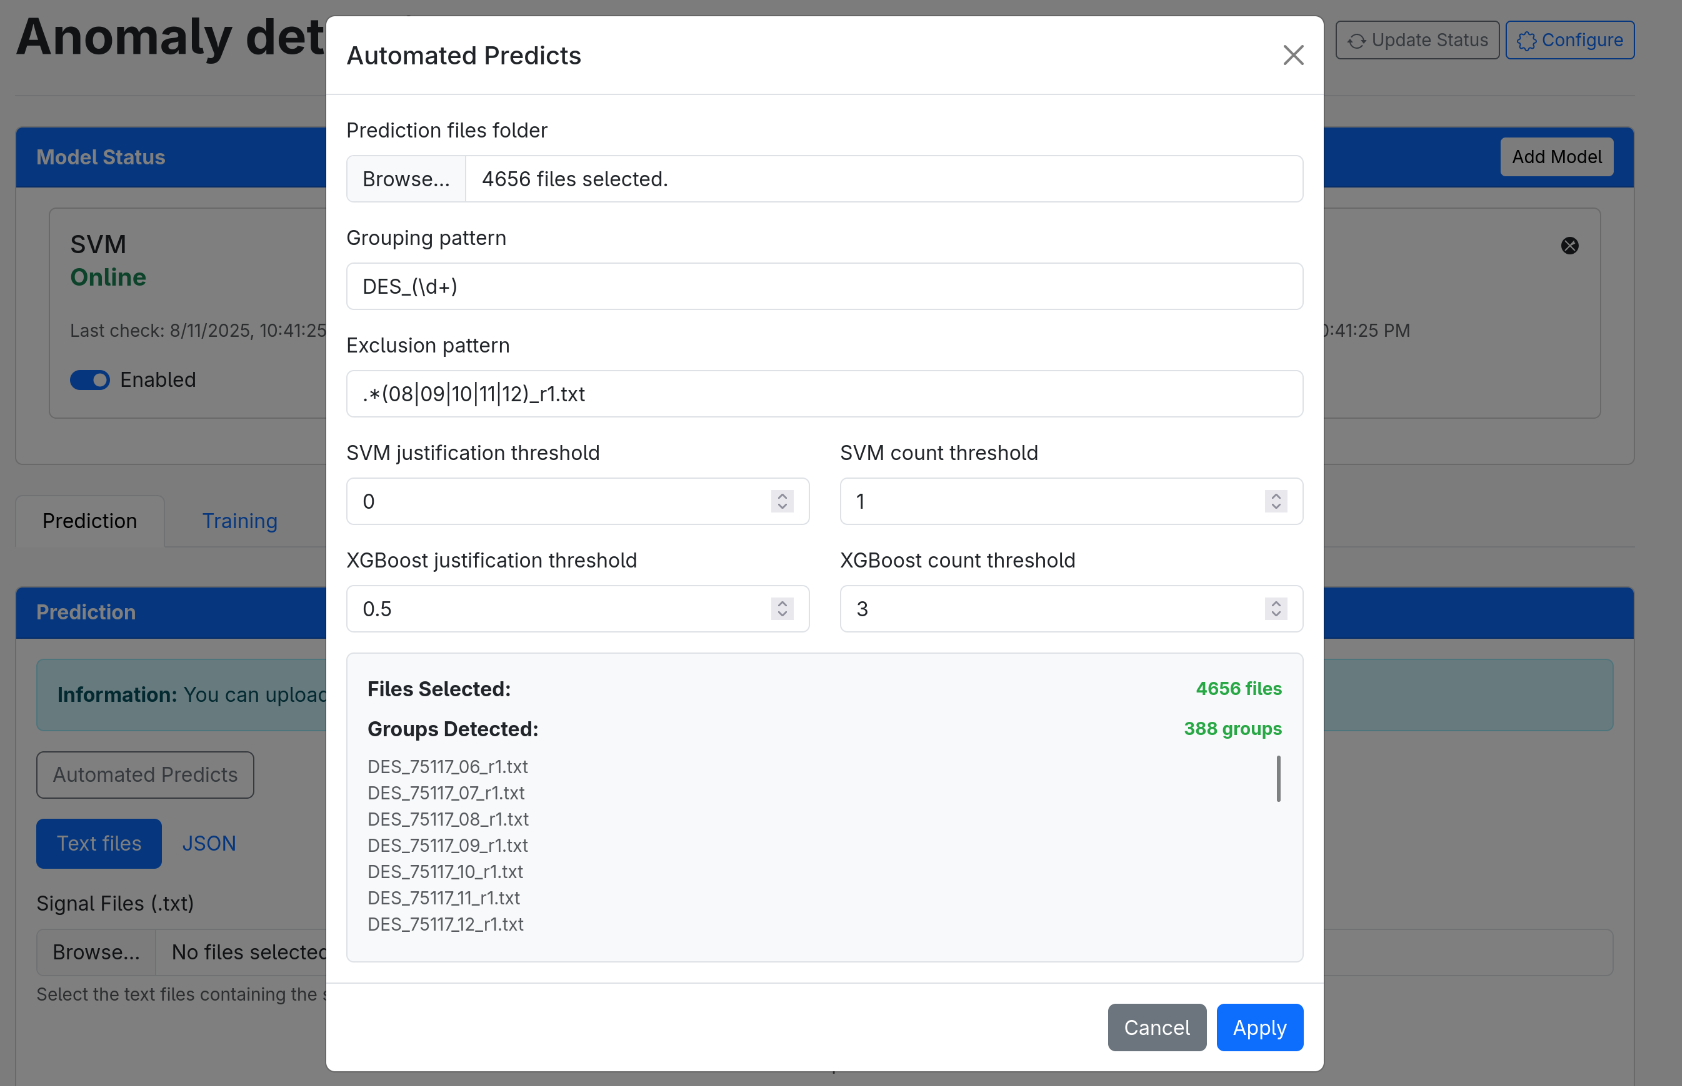
\includegraphics[width=\textwidth]{frontend-automated-predicts.png}
    \caption{Automated predictions}
    \label{fig:auto-pred}
\end{figure}

\subsubsection{Training Tab}

The training tab (\autoref{fig:frontend-training}) is similar to the prediction tab, but users shall select more than one discharge to train the models. For simplicity, there is a button that allow to add multiple discharges at once, opening a modal that allows to select multiple input files, group them using a custom regular expression, and exclude some files with another regular expression. This modal is shown in \autoref{fig:frontend-add-multiple-discharge}. Discharges can also be labeled as disruptive or non-disruptive by setting a disruption time.

\begin{figure}[H]
    \centering
    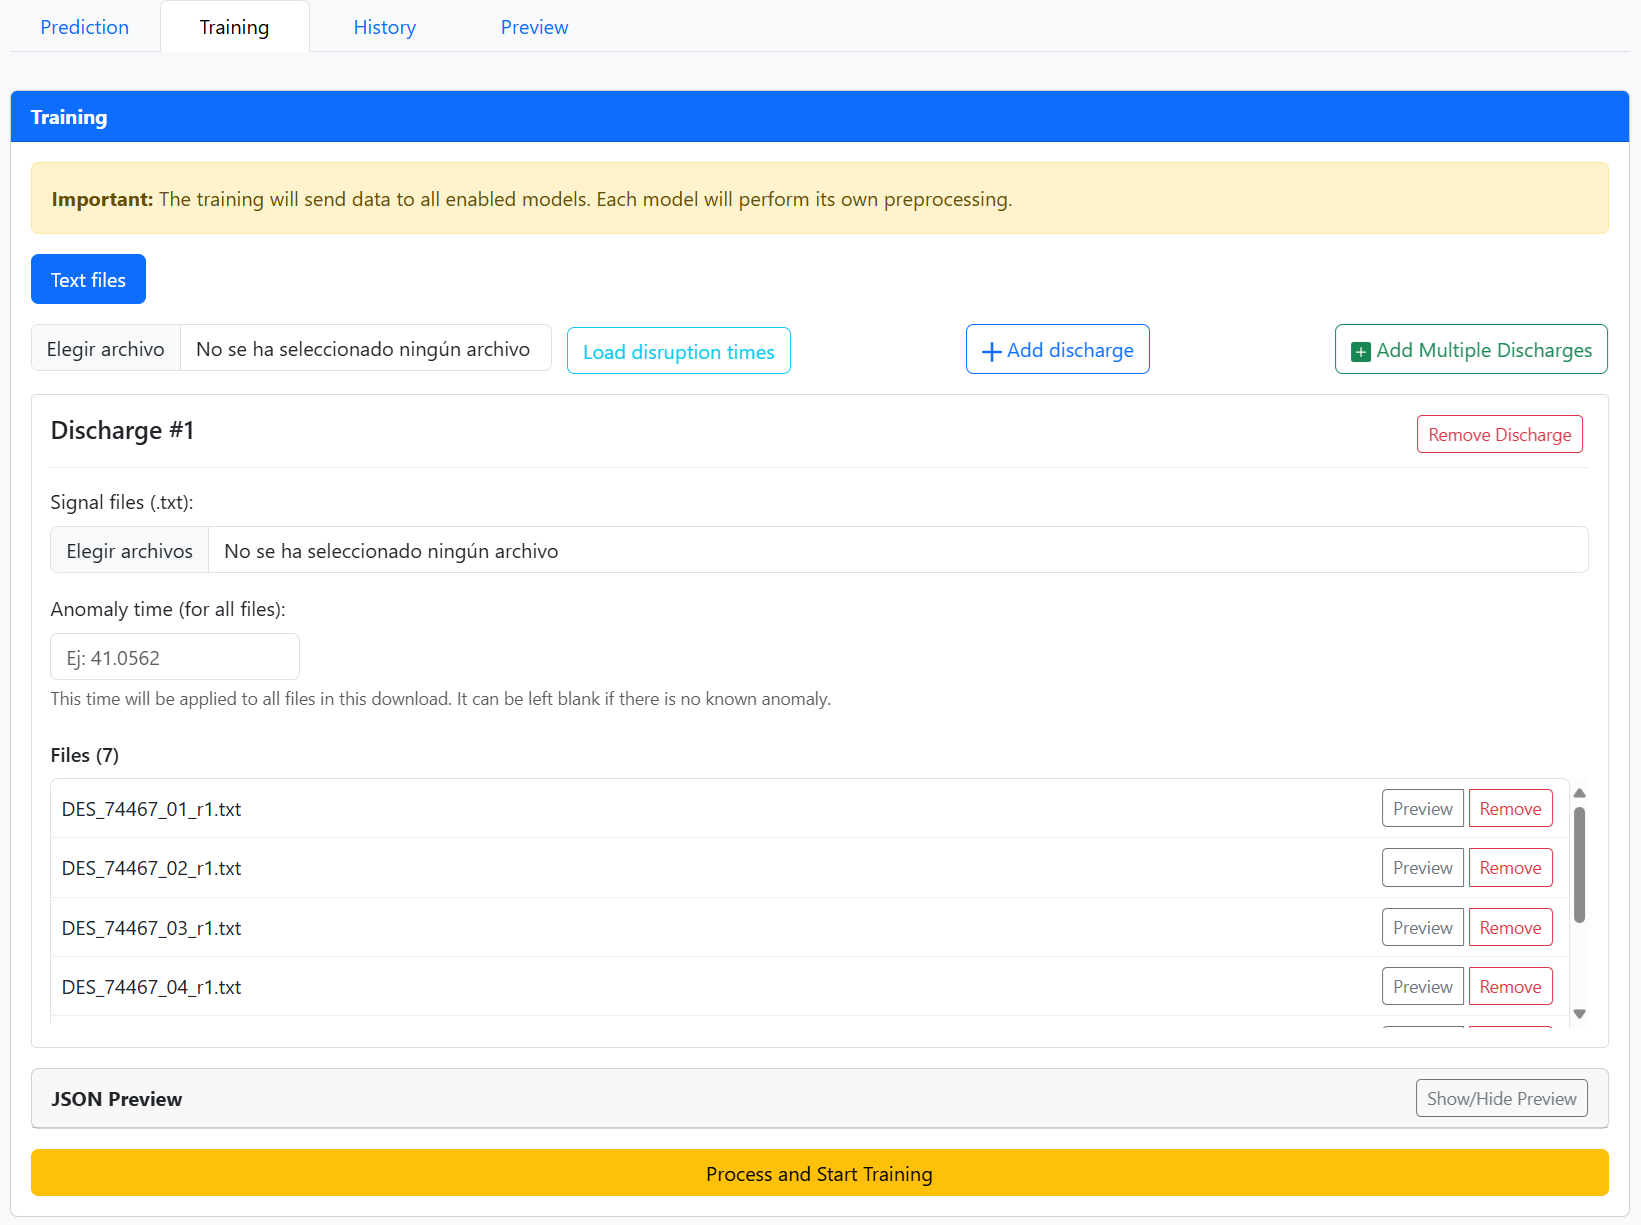
\includegraphics[width=\textwidth]{frontend-train.png}
    \caption{Frontend training tab}
    \label{fig:frontend-training}
\end{figure}

\begin{figure}[H]
    \centering
    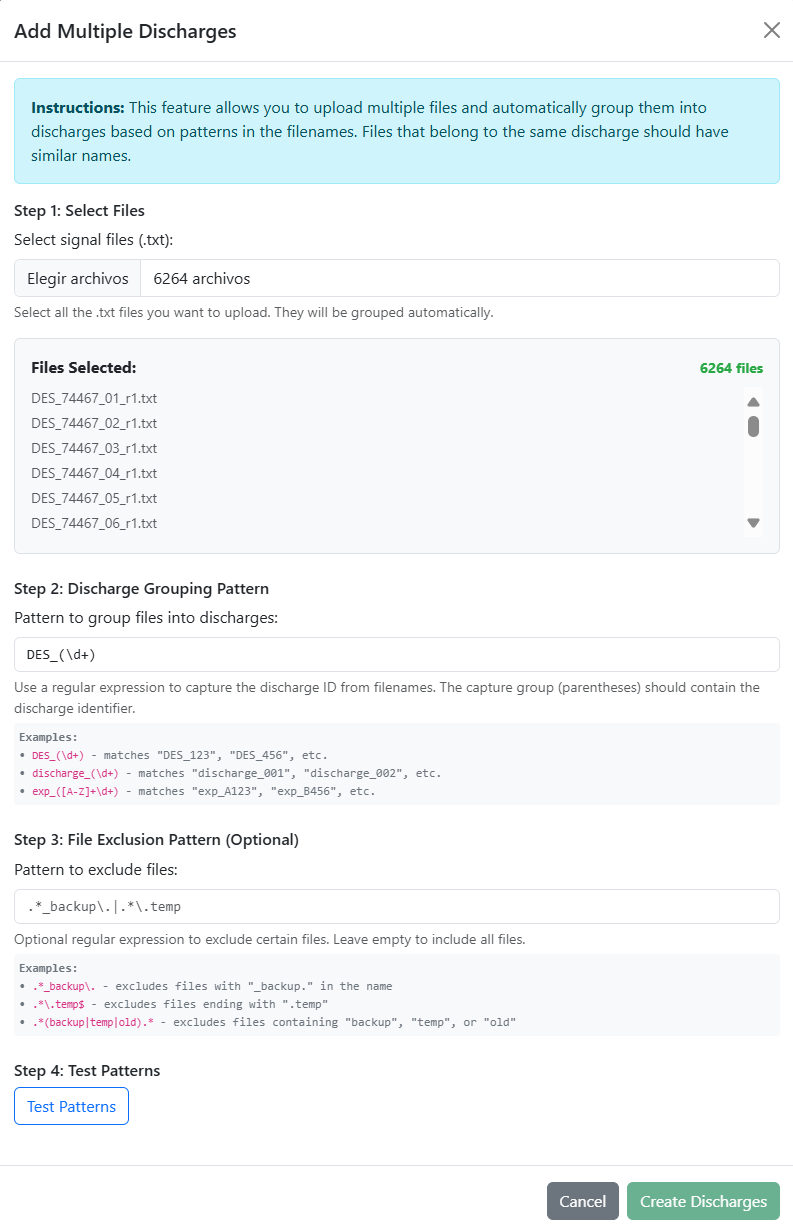
\includegraphics[width=0.5\textwidth]{multiple-discharge-modal.png}
    \caption{Add multiple discharges modal}
    \label{fig:frontend-add-multiple-discharge}
\end{figure}

\subsection{Backend}

The orchestrator's backend implementation is complex, as has to handle every possible message from the models. 

The orchestrator backend has three main components: the controller, the middleware and the services. 

The controller is a high-level class that stores model-related information, such as the current alive models, the prediction output, or the training process. It has advanced features for being efficient in memory usage, as queues to store just the necessary files while training. This feature is explained below.

The middleware is a group of utilities to validate input and output information. When the controller sends an order to the models, middleware ensures that information is well-formed to ensure compatibility. It also works on the other way, as model's messages are validated throw the middleware. This component guarantees that if an error occurs, it does not propagate and leads to undefined behavior.

The services component implements the low-level functionality that controller needs to communicate with the models, and exposes a high-level API that controller uses. This component includes the implementation of the voting mechanism, the batching feature to optimize memory usage or the training responses of models.

\subsubsection{Queuing and memory optimization}

The orchestrator is designed to handle multiple models and discharges simultaneously. As a training set can be large (thousands of discharges, each with thousands of windows), the orchestrator does not load every discharge into memory at once. Instead, one queue per model is created, where discharges are stored if needed, freeing memory when possible. The flow is as follows:

\begin{enumerate}
    \item User uploads training files in the dashboard interface through file input or drag-and-drop
    \item Frontend batches files into groups of 10 discharges to avoid overwhelming the server
    \item Frontend creates metadata containing total discharge count and batch discharge information
    \item Frontend sends an HTTP POST request to backend's \texttt{/api/train/raw} endpoint with the batch
    \item Controller receives batch and parses metadata to extract discharge information and file mappings
    \item Controller checks for existing training session or creates new one if none exists
    \item Controller starts a training session, which contacts all enabled models to initialize training
    \item Models respond with acceptance and each gets assigned a queue structure with sequence tracking
    \item Training session object is created with total discharge count, model queues, and processed discharge tracking
    \item Controller processes the current batch of discharges
    \item Service creates lazy stream generator that processes one discharge at a time from the batch
    \item Generator parses sensor files for each discharge individually, not loading all at once
    \item Each processed discharge added to all model queues simultaneously for parallel processing
    \item Discharge memory immediately released after being cloned to all model queues
    \item Asynchronous queue processors start for each model independently and concurrently
    \item Each model's queue processor sends discharges sequentially to that model's training endpoint
    \item Discharge memory released again after successful transmission to each model
    \item Queue processor continues until its queue is empty, then becomes idle
    \item Process repeats for each batch until all discharges sent
    \item Training session monitors progress and automatically finishes when total discharge count reached
    \item All queues emptied and training session cleaned up
    \item Models complete training and send completion notifications back to orchestrator.
\end{enumerate}


\subsubsection{Automated predicts and report generation}

As explained on the frontend section, to facilitate the prediction process, the orchestrator has a built-in feature that allows automatic predictions. This feature loads a directory and makes sequential predictions for each discharge. Orchestrator groups the files by a regular expression, and sends the discharges to the models one by one. Then, orchestrator stores the results and builds a report with statistical data. These results include raw outputs (prediction output per discharge), and a CSV grouping individual window predictions. Results are explained in \autoref{sec:cap4}. The implementation of this feature

\section{Outlier Models}\label{sec:models}

Every model node shall implement the outlier protocol in order to communicate with the orchestrator. This means that every model is a microservice implementing a server that exposes the necessary endpoints to the orchestrator. The models can be implemented in any programming language, as long as they can handle HTTP requests and responses. Models in this project are implemented in Python and Rust.

For compatibility reasons, every model must split discharges in windows of a fixed length (32 points per window). Models are allowed to extract any relevant data from the windows set.

\subsection{Supervised Binary Classification}

\subsubsection{\acs{SVM}}\label{sec:svm}

This project implements a \ac{SVM} model for anomaly detection, which is trained on both disruptive and non-disruptive discharges. The model is implemented in pure Rust, implementing the outlier protocol using the \texttt{actix\_server} framework for the comunication with the orchestrator's backend, and the \texttt{linfa} crate for the \ac{SVM} implementation. 

The model extracts two features from the discharges: the mean value of the plasma current and the \ac{FFT} of the plasma current. This model can be used to classify with a very low number of training samples, and it can also be used for real-time predictions.

\subsubsection{XGBoost}\label{subsubsec:xgboost}

The XGBoost model is implemented in Python, using the \texttt{xgboost} library for the model, and the \texttt{fastapi} framework for the API.\ It is a supervised binary classification model that uses different features extracted from the discharges. These features include basic statics, like the mean and the mean of the slope of each window, the log of the \ac{RMS}, and dynamic features, like the maximum slope, and data related to the second derivative of each window (minimum, maximum and mean). In total, the model uses 7 features extracted from the discharge data for each window.

Model is also fed with the past features of the discharge, that are used as a tendency to give the model more context about the discharge. This means that the model needs a minimum number of windows to be able to make predictions, which is set to 3 windows by default. As past features are treated like the current features, the model uses a total of 28 features (7 features per window, and 4 windows).

The necessary parameters to create an XGBoost model with the \texttt{xgboost} library are shown on \autoref{lst:xgboost-params}. These parameters are set to values that have been tested and work well for the project, but they can be modified to improve the model's performance. The \texttt{tree\_method} is set to \texttt{hist} to use a histogram-based algorithm, which is faster and more memory-efficient than the default \texttt{exact} method\todo{Ref}. The \texttt{n\_jobs} parameter is set to -1 to use all available CPU cores for training. The \texttt{objective} is set to \texttt{binary:logistic} for binary classification, and the evaluation metric is set to \texttt{aucpr} (area under the precision-recall curve) for better performance in imbalanced datasets, like the given ones. 

\begin{lstlisting}[language=Python, caption={XGBoost model parameters}, label={lst:xgboost-params}]
    params = {
        # Algorithm and hardware settings
        'tree_method': 'hist',
        'n_jobs': -1,
        # Objective and evaluation metrics
        'objective': 'binary:logistic',
        'eval_metric': 'aucpr',
        # Regularization and overfitting control
        'learning_rate': 0.05,
        'scale_pos_weight': scale_pos_weight,
        # Hyperparameters
        'max_depth': 6,
        'min_child_weight': 3,
        'gamma': 1.0,
        'eta': 0.02,
        'subsample': 0.8,
        'colsample_bytree': 0.8,
    }

    dtrain = xgb.DMatrix(X_array, label=y_array)
    model = xgb.train(params, 
                      dtrain, 
                      num_boost_round=10000, 
                      verbose_eval=10
                      )

\end{lstlisting}

XGBoost predicts the probability of a window being disruptive, so a post-processing step is needed to determine if the discharge is disruptive or not. This post-processing step is done by setting a threshold, which is set to 0.5 by default, and a number of consecutive windows that must be disruptive to consider the discharge as disruptive, which is set to 3 by default. This means that if 3 consecutive windows are above the threshold, the discharge is considered disruptive.



\subsubsection{CNN-FFT}

\subsection{Outlier Detection}

This section explains outlier detection models that are implemented for the project. These models are only trained with non-disruptive discharges, and try to find common patterns between them. If a window differs more than a threshold from the pattern, it is labeled as disruptive.

\subsubsection{\acs{OC-SVM}}

\subsubsection{Isolation Forest}

The \ac{IForest} model is implemented in Python, using \texttt{sklearn} library for the model, and the \texttt{fastapi} framework for the API.\ As \texttt{sklearn} is used, if a \ac{GPU} is available, it will be used to improve training times.

This model extracts some relevant features from windows, which include statistical data (mean value, standard deviation, minimum, maximum and range)

\subsubsection{\acs{LSTM}}

